\chapter{Background: Ionizing Radiation}
\label{chap:backgroundsources}

\begin{changemargin}{1.0cm}{1.0cm}
\abstractpreamble{There are a wide range of radiation sources and types of ionising radiation.  They interact differently with matter, depending on the type of radiation and its energy.  Damage may be caused with the radiation transferring energy directly to the target.  The target may be transmuted or the surrounding, for example the creation of Cobalt-60 in steel in the nuclear industry.  The environment may be changed chemically, and one example of this is the radiolysis of water.}
\end{changemargin}



%%%%%%%%%%%%%%%%%%%%%%%%%%%%%%%%%%%%%%%%%%%%%%%%%%%%%%%%%%%%%%%%%%%%%%%%%%%%%%%%%%%%%%%%%%%%%%%%%%%%%%%%%%
%%
%%  RADIATION TYPES
%%
%%%%%%%%%%%%%%%%%%%%%%%%%%%%%%%%%%%%%%%%%%%%%%%%%%%%%%%%%%%%%%%%%%%%%%%%%%%%%%%%%%%%%%%%%%%%%%%%%%%%%%%%%%


\section{Radiation Types Relevant to This Work}


\subsection{Introduction}

There are three types of radiation that are useful to discuss in this work, neutrons, ions and Ggammas, and two of these (neutrons and protons) are of particular interest in this work.  Each of these are capable of ionizing the atoms they interact with, given sufficient energy.  Higher energy and momentum radiation it is able to directly damage materials, or the \acrshort{dna} structure of organic life, that it interacts with.  Lower momentum ionizing radiation may change the water chemistry of the environment or within the cells of organic lifeforms that is detrimental to life.



\subsection{Protons and other Ions}

Charged particles interact with matter through the Coulomb interaction.  As a charged particle passes through matter, it may interact with both the nucleus and electrons of an atom.  A sufficiently energetic ion may lose kinetic energy to electrons by either raising the electrons to higher energy levels in their atoms, or by removing electrons from atoms altogether, causing the ionization of those atoms.  

Ions may also lose kinetic energy to the nucleus of an atom through elastic scattering and, where the atom is in a crystal structure, through knocking atoms in the material out of their lattice positions.  Inelastic scattering is also a possibility, leaving the target nucleus in an excited state.

Knock on atoms and electrons with enough kinetic energy that have been removed from atoms (delta rays), continue the irradiation of the material while they have the kinetic energy available to do so.

A large proportion of the energy of a charged projectile is lost to the electrons of the target material.  There is a chance, depending on the energy and type of charged projectile (and the cross section of the target nucleus), that the charged particle will overcome the coulomb potential and be captured by the nucleus.

This may result in a stable nucleus or an unstable nucleus.  If it is unstable, there is a probability that it will decay releasing energy in the form of photons, nucleons or electrons.  The initial ion irradiation creates sources of further radiation within the target material.



\FloatBarrier
\subsection{Neutrons}


Neutrons interact with matter differently to that of protons, ions and other atoms, as the neutron has no overall charge.  Neutrons do have a magnetic moment and experience a weak interaction with unpaired electrons by a dipole-dipole interaction.  Neutrons also interact with the nucleus of atoms, and this is dependant upon the target atom and the energy of the projectile neutron.  The energy of neutrons may be grouped as shown in table \ref{table:neutronenergies}, and as mentioned earlier, thermal neutrons are of interest to current reactor designs, and fast neutrons are of interest to several future designs.
 
\begin{table}[h]
\begin{center}
\renewcommand{\arraystretch}{1.2}
\begin{tabular}{c c c c}
\hline\hline
Name & Energy Range & Velocity/ms\textsuperscript{-1} & Wavelength Ang \\
\hline\hline
Cold & 0-0.025 eV & 0.0 - $2.2 \times 10^{3}$ &  $> 1.8$  \\
Thermal & 0.025 eV & ~$2.2 \times 10^{3}$ &  1.8  \\
Epithermal & 0.025-0.4 eV & $2.2 \times 10^{3}$ - $8.8 \times 10^{3}$ &  0.5-1.8 \\
Cadmium & 0.4-0.6 eV & $8.8 \times 10^{3}$ - $1.1 \times 10^4$ & 0.4-0.5  \\
Epicadmium & 0.6-1.0 eV & $1.1 \times 10^4$ - $1.4 \times 10^4$ & 0.3-0.4\\
Slow & 1-10 eV & $1.4 \times 10^4$ - $4.4 \times 10^4$   & 0.09-0.3\\
Resonance & 10-300 eV & $4.4 \times 10^4$ - $2.4 \times 10^5$ & 0.02-0.09\\
Intermediate & 300 eV - 1 MeV &  $2.4 \times 10^5$ & $2.9 \times 10^{-4}$ - $0.02$\\
Fast & 1-20 MeV & $1.4 \times 10^7$ - $6.1 \times 10^7$ & $6.5 \times 10^{-5}$ - $2.9 \times 10^{-4}$ \\
Relativistic & $>20$ MeV & $>6.1 \times 10^{7}$ & $< 6.5 \times 10^{-5}$\\
\hline\hline
\end{tabular}
\end{center}
\caption{Neutron Categories by Energy Range \cite{njcarron}}
\label{table:neutronenergies}
\end{table}

The nuclear force holds nuclei together by exchanging pions.  It is 137 times stronger than the electromagnetic force, but because of the mass of the pion (approximately 130-140MeV) it only acts over a short range of approximately 1fm.  The nuclear force is attractive but has a short-range repulsive core.


\begin{figure}
\centering
\begin{minipage}{.30\textwidth}
\centering
\begin{tikzpicture}
  \begin{feynman}
    \vertex (a) {\(p\)};
    \vertex [below right=of a] (b);
    \vertex [above right=of b] (c) {\(p\)};
    \vertex [below right=of b] (d);
    \vertex [below left=of d] (f) {\(p\)};
    \vertex [below right=of d] (g) {\(p\)};
    \diagram* {
      (a) -- [fermion] (b),
      (b) -- [fermion] (c),
      (b) -- [scalar, edge label=\(\Pi^{0}\)] (d),
      (f) -- [fermion] (d),
      (d) -- [fermion] (g),
    };
  \end{feynman}
\end{tikzpicture}
\caption{Direct interaction p-p\cite{pionexchange}}
\label{fig:pppion}
\end{minipage}
\begin{minipage}{.30\textwidth}
\centering
\begin{tikzpicture}
  \begin{feynman}
    \vertex (a) {\(p\)};
    \vertex [below right=of a] (b);
    \vertex [above right=of b] (c) {\(p\)};
    \vertex [below right=of b] (d);
    \vertex [below left=of d] (f) {\(n\)};
    \vertex [below right=of d] (g) {\(n\)};
    \diagram* {
      (a) -- [fermion] (b),
      (b) -- [fermion] (c),
      (b) -- [scalar, edge label=\(\Pi^{0}\)] (d),
      (f) -- [fermion] (d),
      (d) -- [fermion] (g),
    };
  \end{feynman}
\end{tikzpicture}
\caption{Direct interaction p-n\cite{pionexchange}}
\label{fig:pnpion}
\end{minipage}
\begin{minipage}{.30\textwidth}
\centering
\begin{tikzpicture}
  \begin{feynman}
    \vertex (a) {\(n\)};
    \vertex [below right=of a] (b);
    \vertex [above right=of b] (c) {\(n\)};
    \vertex [below right=of b] (d);
    \vertex [below left=of d] (f) {\(n\)};
    \vertex [below right=of d] (g) {\(n\)};
    \diagram* {
      (a) -- [fermion] (b),
      (b) -- [fermion] (c),
      (b) -- [scalar, edge label=\(\Pi^{0}\)] (d),
      (f) -- [fermion] (d),
      (d) -- [fermion] (g),
    };
  \end{feynman}
\end{tikzpicture}
\caption{Direct interaction n-n\cite{pionexchange}}
\label{fig:nnpion}
\end{minipage}
\end{figure}


\begin{figure}
\centering
\begin{minipage}{.30\textwidth}
\centering
\begin{tikzpicture}
  \begin{feynman}
    \vertex (a) {\(p\)};
    \vertex [below right=of a] (b);
    \vertex [above right=of b] (c) {\(n\)};
    \vertex [below right=of b] (d);
    \vertex [below left=of d] (f) {\(n\)};
    \vertex [below right=of d] (g) {\(p\)};
    \diagram* {
      (a) -- [fermion] (b),
      (b) -- [fermion] (c),
      (b) -- [scalar, edge label=\(\Pi^{+}\)] (d),
      (f) -- [fermion] (d),
      (d) -- [fermion] (g),
    };
  \end{feynman}
\end{tikzpicture}
\caption{Exchange interaction n-p\cite{pionexchange}}
\label{fig:pppion}
\end{minipage}
\begin{minipage}{.30\textwidth}
\centering
\begin{tikzpicture}
  \begin{feynman}
    \vertex (a) {\(n\)};
    \vertex [below right=of a] (b);
    \vertex [above right=of b] (c) {\(p\)};
    \vertex [below right=of b] (d);
    \vertex [below left=of d] (f) {\(p\)};
    \vertex [below right=of d] (g) {\(n\)};
    \diagram* {
      (a) -- [fermion] (b),
      (b) -- [fermion] (c),
      (b) -- [scalar, edge label=\(\Pi^{-}\)] (d),
      (f) -- [fermion] (d),
      (d) -- [fermion] (g),
    };
  \end{feynman}
\end{tikzpicture}
\caption{Exchange interaction p-n\cite{pionexchange}}
\label{fig:pnpion}
\end{minipage}
\end{figure}

For nuclear reaction and damage calculations, the interaction of neutrons with matter is represented by a cross section (section \ref{section:nuclearxs}).  Cross sections are used to calculate the probability of a certain interaction occurring and are dependent upon the target nucleus, how much of the material the pass through and the energy of the neutron.

The attenuation of neutron radiation is therefore a complicated process.  A much larger thickness of shielding is required to stop neutrons, or at least bring them to thermal temperatures.  Not only this, but the thermalized neutrons must then be captured.  During this process various isotopes within the attenuating shielding will have been transmuted, possibly into radioactive isotopes.  As a rough estimate if a certain amoint of material will attenuate neutrons to 10\% their original flux, then the same amount of material will reduce the flux further to 1\%.  This is however an over simplification and computer codes such as \acrfull{mcnp} and TART more accurately model the transport of neutrons through materials. 



\FloatBarrier
\subsection{High Energy Photons}

The electromagnetic spectrum classifies photons based on their energy and/or source, but visible light, x-rays, gamma rays and so on are all the same elementary \enquote{particle}.  During the early years of Quantum Mechanics, the relationship between the energy and wavelength of a photon was discovered: the Planck-Einstein relation (eq. \ref{eq:planckeinstein}).

\begin{equation}
\begin{split}
E = h f
\end{split}
\label{eq:planckeinstein}
\end{equation}

\subsubsection{Pair Production}

The energy of photons in the database used for this work ranges from 1keV up to almost 10MeV.  There are several ways high energy photons will interact with the atoms of a target material.  The rest mass of an electron is 511keV.  If the photon energy is greater than 1.02MeV, i.e. there is at least enough energy to create an electron and positron, there is a chance that the photon will create an electron-proton pair.  

\begin{equation}
\begin{split}
h f = (m_e + m_p) c^2 + T_e + T_p
\end{split}
\end{equation}

The creation conserves energy and mass, with excess energy carried away as the kintetic energy of the particle pair.  The charge before the creation is zero, as the photon is neutral, and the charge after is also zero, with the -1 of the electron and +1 of the positron cancelling out.  Angular momentum is also conserved; the photon is a spin 1 Boson and, as electrons and positrons are Leptons they have half integer spin, adding up to 1.  Finally, momentum is not conserved in a vacuum, and this is why pair production occurs in the coulomb field of a nucleus.  The nucleus carries away excess momentum, fulfilling this conservation law (fig. \ref{fig:pairproduction}).

\begin{figure}[h]
\begin{center}
\begin{tikzpicture}
  \begin{feynman}
    \vertex (a) {\(\gamma\)};
    \vertex [right=of a] (b);
    \vertex [above right=of b] (c) {\(e^-\)};
    \vertex [below right=of b] (d);
    \vertex [below right=of d] (e) {\(e^+\)};
    \vertex [below =of d] (f);
    \vertex [below left=of f] (g) {\(Z\)};
    \vertex [below right=of f] (h) {\(Z\)};
    \diagram* {
      (a) -- [boson] (b),
      (b) -- [fermion] (c),
      (b) -- [fermion] (d),
      (d) -- [fermion] (e),
      (d) -- [boson] (f),
      (g) -- [fermion] (f),
      (f) -- [fermion] (h),
    };
  \end{feynman}
\end{tikzpicture}
\end{center}
\caption{Pair production Feynman diagram}
\label{fig:pairproduction}
\end{figure}


\subsubsection{Compton Scattering}

An incident photon with enough energy may interact with the electron of an atom, and if it transfers enough kinetic energy it will eject the electron from the atom (fig. \ref{fig:comptonscattering}).  A lower energy photon is also created that carries away the remainder of the energy, but also linear momentum, as both energy and momentum must be conserved.

\begin{figure}[h]
\begin{center}
\begin{tikzpicture}
  \begin{feynman}
    \vertex (a) {\(\gamma\)};
    \vertex [below right=of a] (b);
    \vertex [right=of b] (c);
    \vertex [below left=of b] (d) {\(e^{-}\)};
    \vertex [above right=of c] (e) {\(\gamma\)};
    \vertex [below right=of c] (f) {\(e^{-}\)};
    \diagram* {
      (a) -- [boson] (b),
      (b) -- [fermion] (c),
      (d) -- [fermion] (b),
      (c) -- [boson] (e),
      (c) -- [fermion] (f),
    };
  \end{feynman}
\end{tikzpicture}
\end{center}
\caption{Compton Scattering Feynman diagram}
\label{fig:comptonscattering}
\end{figure}


\subsubsection{Photoelectric Effect}

Photons of sufficient energy interact with and eject electrons from the surface of a metal (fig. \ref{fig:photoelectric}).  At lower energies, the photons have no effect on the electrons.  Ejected electrons have a maximum kinetic energy equal to the difference between the energy of the interacting photon and the workfunction, $T_{max} = h \nu - \phi$.

\begin{figure}[h]
\begin{center}
\begin{tikzpicture}
  \begin{feynman}
    \vertex (a) {\(\gamma\)};
    \vertex [below right=of a] (b);
    \vertex [right=of b] (c);
    \vertex [below left=of b] (d) {\(Z_{n}^{+},e_{n}^{-}\)};
    \vertex [above right=of c] (e) {\(e_{1}^{-}\)};
    \vertex [below right=of c] (f) {\(Z_{n}^{+},e_{n-1}^{-}\)};
    \diagram* {
      (a) -- [boson] (b),
      (b) -- [fermion] (c),
      (d) -- [fermion] (b),
      (c) -- [fermion] (e),
      (c) -- [fermion] (f),
    };
  \end{feynman}
\end{tikzpicture}
\end{center}
\caption{Photoelectric Effect Feynman diagram}
\label{fig:photoelectric}
\end{figure}



\subsubsection{Coherent Scattering}

Lower energy, non-ionizing photons, have insufficient energy to eject electrons (fig. \ref{fig:coherentscattering}).  Coherent scattering is the interaction in which photons change direction, scattering, without losing energy. 


\begin{figure}[h]
\begin{center}
\begin{tikzpicture}
  \begin{feynman}
    \vertex (a) {\(\gamma\)};
    \vertex [below right=of a] (b);
    \vertex [right=of b] (c);
    \vertex [below left=of b] (d) {\(Z^{+}\)};
    \vertex [above right=of c] (e) {\(\gamma\)};
    \vertex [below right=of c] (f) {\(Z^{+}\)};
    \diagram* {
      (a) -- [boson] (b),
      (b) -- [fermion] (c),
      (d) -- [fermion] (b),
      (c) -- [boson] (e),
      (c) -- [fermion] (f),
    };
  \end{feynman}
\end{tikzpicture}
\end{center}
\caption{Coherent Scattering Feynman diagram}
\label{fig:coherentscattering}
\end{figure}

\subsubsection{Gamma Attenuation}

Whilst an infinite amount of material is required to reduce the intensity of gammas to zero, they may be reduced by a significant amount with dense material.  Lead, Uranium and other dense materials with a large number of electrons per unit volume are ideal.

\begin{equation}
\begin{split}
I(\mu/\rho(E), t) = I_0 exp\left(\frac{-\mu}{\rho}(E) \rho t \right)
\end{split}
\label{eq:knollattenuation}
\end{equation}

The attenuation is dependent upon the thickness of the material , with a thicker material reducing the intensity of the gammas (eq. \ref{eq:knollattenuation}\cite{gknollattenuation}).  It is also dependent upon the mass attenuation coefficients that are in turn dependent upon the photon energy.  A table of attenuation coefficients are available for each element\cite{massattenuation}.



\FloatBarrier





%%%%%%%%%%%%%%%%%%%%%%%%%%%%%%%%%%%%%%%%%%%%%%%%%%%%%%%%%%%%%%%%%%%%%%%%%%%%%%%%%%%%%%%%%%%%%%%%%%%%%%%%%%
%%
%%  CROSS SECTIONS
%%
%%%%%%%%%%%%%%%%%%%%%%%%%%%%%%%%%%%%%%%%%%%%%%%%%%%%%%%%%%%%%%%%%%%%%%%%%%%%%%%%%%%%%%%%%%%%%%%%%%%%%%%%%%

\section{Microscopic and Macroscopic Cross Sections}

As discussed above there are a range of different ways in which matter interacts.  The probability that a certain interaction will happen, which may be a function of the target, projectile and projectile energy, is described with the microscopic cross section.  The total microscopic cross section is computed by summing all the individual reaction channels (eq. \ref{eq:totalmicroscopic})

\begin{equation}
\begin{split}
\sigma_{total} = \sigma_{elastic} + \sigma_{inelastic} + \sigma_{absorption} + \sigma_{fission} + \dots
\end{split}
\label{eq:totalmicroscopic}
\end{equation}

The cross section has units of area and is measured in \gls{barn}s.  When this area is multiplied by the target thickness and number density of the target, the fraction of projectiles that will react in this way is computed (see section \ref{section:protonactivation}).

Multiplying the microscopic cross sections by the number density defines the macroscopic cross section, whether it be for an individual reaction type or the sum of them all.  This has units of atoms per meter and taking the inverse gives the \gls{meanfreepath} of the projectile in the target material.

\begin{minipage}[b]{0.49\linewidth}
\begin{center}
\begin{equation}
\begin{split}
\Sigma{total} = N_{d} \times \sigma_{total} \text{    } 
\end{split}
\label{eq:totalmicroscopic}
\end{equation}
\end{center}
\end{minipage}
\begin{minipage}[b]{0.49\linewidth}
\begin{center}
\begin{equation}
\begin{split}
\lambda = \frac{1}{\Sigma}
\end{split}
\label{eq:totalmicroscopic}
\end{equation}
\end{center}
\end{minipage}

The probabilities and associated libraries of a neutron, proton, deuteron and so on transmuting a target atom are discussed in more detail in section \ref{section:nuclearxs}.


\FloatBarrier



%%%%%%%%%%%%%%%%%%%%%%%%%%%%%%%%%%%%%%%%%%%%%%%%%%%%%%%%%%%%%%%%%%%%%%%%%%%%%%%%%%%%%%%%%%%%%%%%%%%%%%%%%%
%%
%%  Quantifying Radiation
%%
%%%%%%%%%%%%%%%%%%%%%%%%%%%%%%%%%%%%%%%%%%%%%%%%%%%%%%%%%%%%%%%%%%%%%%%%%%%%%%%%%%%%%%%%%%%%%%%%%%%%%%%%%%

\section{Quantifying Radiation and its Effects}

The reason for attributing a value to a radiation source is usually because we want to quantify it and link that value to the effects it will have on materials, equipment and, most importantly, people.  There are a number ways of quantifying radiation, an associated number of different units as well as many other factors that affect how concerned we should be about a particular source.

Parameters most obvious to quantify radiation are the rate at which the particles are being created as well as the duration the equipment, material or person is exposed to that radiation. 

The energy of the particles will determine the type of damage it is able to do.  We are regularly exposed to visible light with several hundred watts or more per square meter courtesy of the Sun.  The same power from a 1-2MeV gamma source would require far fewer photons, with a million visible light photons for every gamma, but the affect wouldn't be a gentle warming as it would be for sunlight, but a fatal dose of radiation.

How far the radiation is able to travel is another factor as a certain dose may be received very close to the source, but reduced due to both spherical degradation and attenuation at a distance further away.  This is particularly relevant for charged particle radiation such as alphas and betas.

The material, component or part of the body radiation passes through will also determine its effect.  Some parts of the body are more sensitive to radiation that others.


% and a comparison is given in table \label{table:dosecomparison}.
%tissue weigting table


Radioactivity, the number of decays per second, is measured in either \Gls{becquerel}, \Gls{curie} or \gls{rutherford}.  The Curie was based on the radioactivity of Radon-226, but for the most of this work, the unit of choice will be \gls{becquerel}.

Fluence ($\phi$) is the measure of the total number of particles passing through an area (eq. \ref{eq:fluence}).  Whilst this is typically defined as the amount passing through a spherical area, the proton radiation that concerns this work is directional and it will be the planar fluence\cite{dosimetrygreening}.  The fluence rate is a measure of how many particles pass through a sphere (or plane where planar) per second.

\begin{equation}
\begin{split}
\phi = N/A \text{    } \dot{\phi} = \frac{d\phi}{dt} 
\label{eq:fluence}
\end{split}
\end{equation}

Absorbed dose is the amount of energy absorbed by a unit mass.  This will be the sum of the fluence and energies of each individual particle and will depend upon the proportion of that energy deposited in the target.  It is measured in the SI unit \gls{gray} although a historical unit is \gls{rad}, which is equal to 1 centigray.

\begin{equation}
\begin{split}
D_{equivalent} = W_{r} \times D_{absorbed} \\
D_{equivalent} = W_{r} \times W_{t} \times D_{absorbed} \\
\label{eq:equivalenteffectivedose}
\end{split}
\end{equation}

Both the type of radiation and the type of tissue determine how much of an impact that radiation has per unit energy per unit mass.  Both the equivalent and effective (eq. \ref{eq:equivalenteffectivedose}) dose are measured in the Si unit \gls{sievert}, and historically they have been measured in \gls{rem} where the base unit is cGy rather than Gy.






\FloatBarrier


%%%%%%%%%%%%%%%%%%%%%%%%%%%%%%%%%%%%%%%%%%%%%%%%%%%%%%%%%%%%%%%%%%%%%%%%%%%%%%%%%%%%%%%%%%%%%%%%%%%%%%%%%%
%%
%%  RADIATION DANGERS
%%
%%%%%%%%%%%%%%%%%%%%%%%%%%%%%%%%%%%%%%%%%%%%%%%%%%%%%%%%%%%%%%%%%%%%%%%%%%%%%%%%%%%%%%%%%%%%%%%%%%%%%%%%%%


\section{Effects of Radiation on Organics}
\label{section:effectsofradiationorg}

In this work the primary types of radiation considered in this work are neutrons, protons and gammas.  The materials damage will be predominantly due to neutrons, protons and cascade atoms.  Damage to humans will be primarily due to gamma rays. 

It is assumed the process causing the damage is screened from humans and that this radiation will no longer be present when the irradiated targets are being handled.  It is also assumed that and beta and alphas will also be screen with the main source of irradiation that poses a threat to humans being gammas.  For this reason more focus will be given to the effect of gammas on humans.



\subsection{Reference Levels of Radiation}

Although a sievert is only one joule per kg, because of the nature of the damage cause by ionising radiation, safe levels are measured in millisieverts per year.  The annual upper limit for the general public is just .  A dose of just 5 Sieverts is enough to kill 50\% of people within 1 month (table \ref{table:dosecomparison}). 

\begin{table}[h]
\begin{center}
\renewcommand{\arraystretch}{1.2}
\begin{tabular}{c c}
\hline\hline
Exposure & Dose (mSv) \\
\hline\hline
Dental X-ray & 0.005 \\
Chest X-ray & 0.02 \\
UK average annual dose limit for the public &  1.0 \\
UK average annual dose (background) &  2.7 \\
Whole bodt CT scan & 10 \\
Nuclear industry employee annual exposure limit & 20 \\
Acute radiation effects & 1,000 \\
50\% lethal dose within 1 month & 5,000 \\
\hline\hline
\end{tabular}
\end{center}
\caption{Irradiation dose comparison in mSv}
\label{table:dosecomparison}
\end{table}

The regulations on ionising radiation\cite{ionisingradiationregulations} also specify limits per square centimetre on skin, where the total dose might be within the annual limit but when concentrated in a small region it could cause damage to that region.  Certain parts of the body also have limits applied, such as the lens of the eye.

\subsection{Levels of Radioactivity from Neutron Irradiated Components}

In work by Rodenas and Verdu a MCNP5 simulated neutron flux environment and a thermal flux of $2.5 \times 10^7 n/cm^2 s$ a stainless steel cylinder (20mm diameter and 70mm depth) was irradiated for 10 hours\cite{radionuclides}.  The sample was composed of 65\% Fe, 19\% Cr, 2.0\% Mn, 1.0\% Si by weight as well are small amounts of C, Ti, P and S.  After 10 minutes cooling, it was calculated to have an activity of over $1.0 \times 10^7$ Bq and, by several orders of magnitude, it was predominantly due to the creation of Mn\textsuperscript{56}.  

The maximum cross section of Mn\textsuperscript{55} (n, $\gamma$) Mn\textsuperscript{56} is 2.0 barns and the estimated reaction rate at this flux is just over $2.0 \times 10^6$.  As the half life of Mn\textsuperscript{56} is short compared to the irradiation time (a half life of 2.5 hours) the creation rate of Mn \textsuperscript{56} and decay rate equalise, saturating the sample with Mn \textsuperscript{56}.

A simple neutron activation code was developed, which will be discussed in more detail in this work, and the predicted Mn\textsuperscript{56} activity vs time was calculated (fig. \ref{fig:mn56activity}).  The overall gamma dose, for 1 minute of exposure to an 80kg person standing 2m from the source was also calculated (fig. \ref{fig:neutron_irradiated_steel_dose1}).  The calculated activity for Mn \textsuperscript{56} was less than that predicted by Rodenas and Verdu \cite{radionuclides}, but it was within an order of magnitude.  It predicts a total activity after cooling of $2.3\times10^6$ Bq with almost 90\% of this due to Mn\textsuperscript{56}.

The flux in the within the flux trap of the HFIR is much higher, with high energy neutrons having a flux of $1.0 \time 10^{14}$ neutrons per cm squared per second (fig. \ref{fig:hfir_neutron_flux}).  A second calculation was performed for this increased flux, also irradiated over 10 hours (fig. \ref{fig:neutron_irradiated_steel_dose2}).  The total activity increased from $2.3\times10^6$ Bq to $7.1\times10^{12}$ Bq and the overall dose per minute was much higher, between 40 and 50 milligrey per minute over the first hour of cooling.  These are dangerous levels of radiation.

\begin{figure}
  \begin{center}
    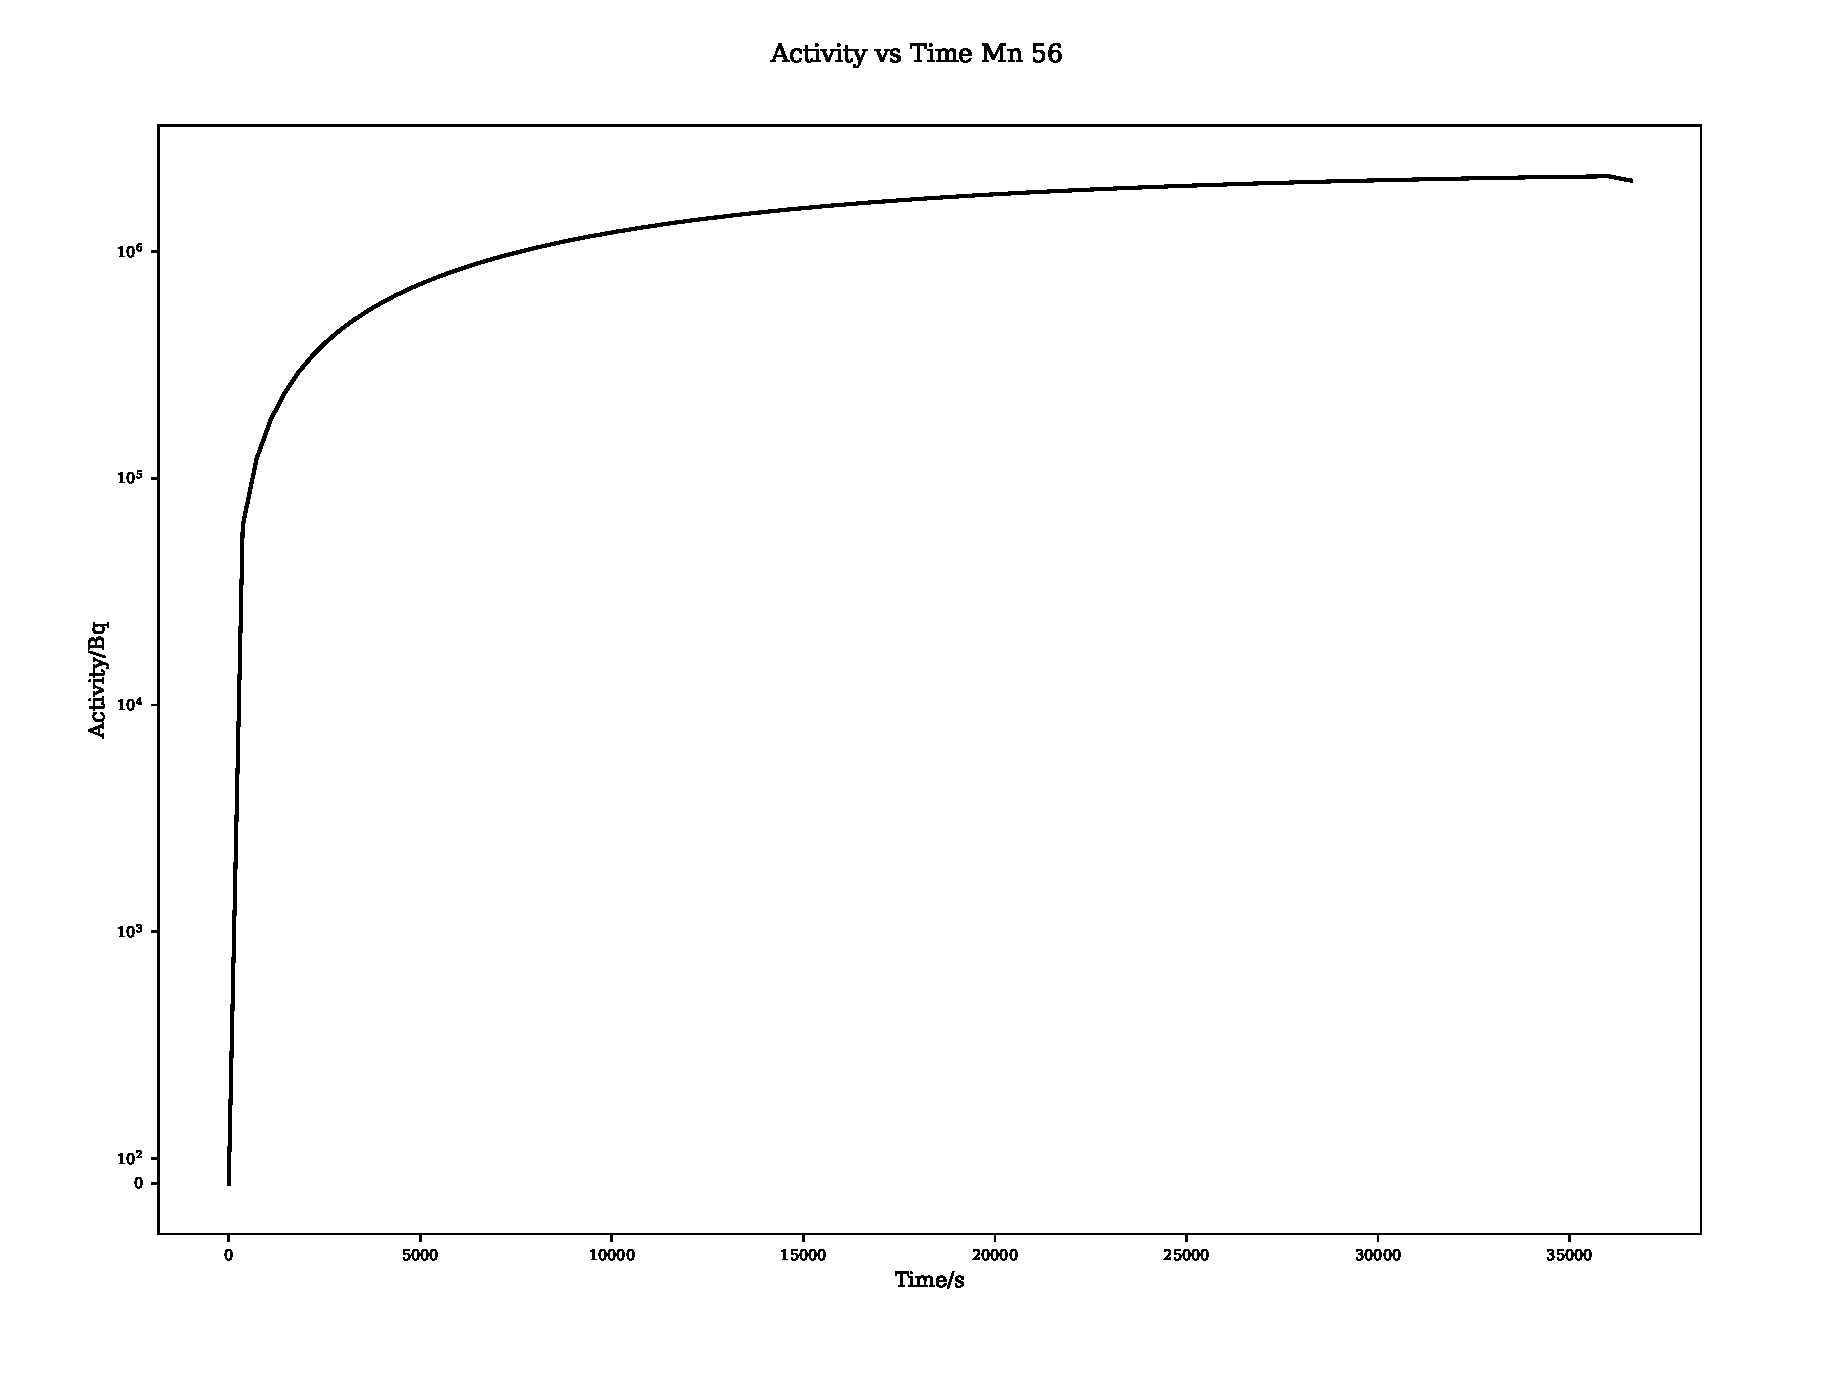
\includegraphics[width=10.0cm]{chapters/background_radiation_effects_and_transport/neutron_plots/1/25_Mn_56_activity.eps}
    \captionsetup{font={it}}
    \caption{Predicted Mn 56 activity after neutron irradiation}
    \label{fig:mn56activity}
  \end{center}
\end{figure}

\begin{figure}
  \begin{center}
    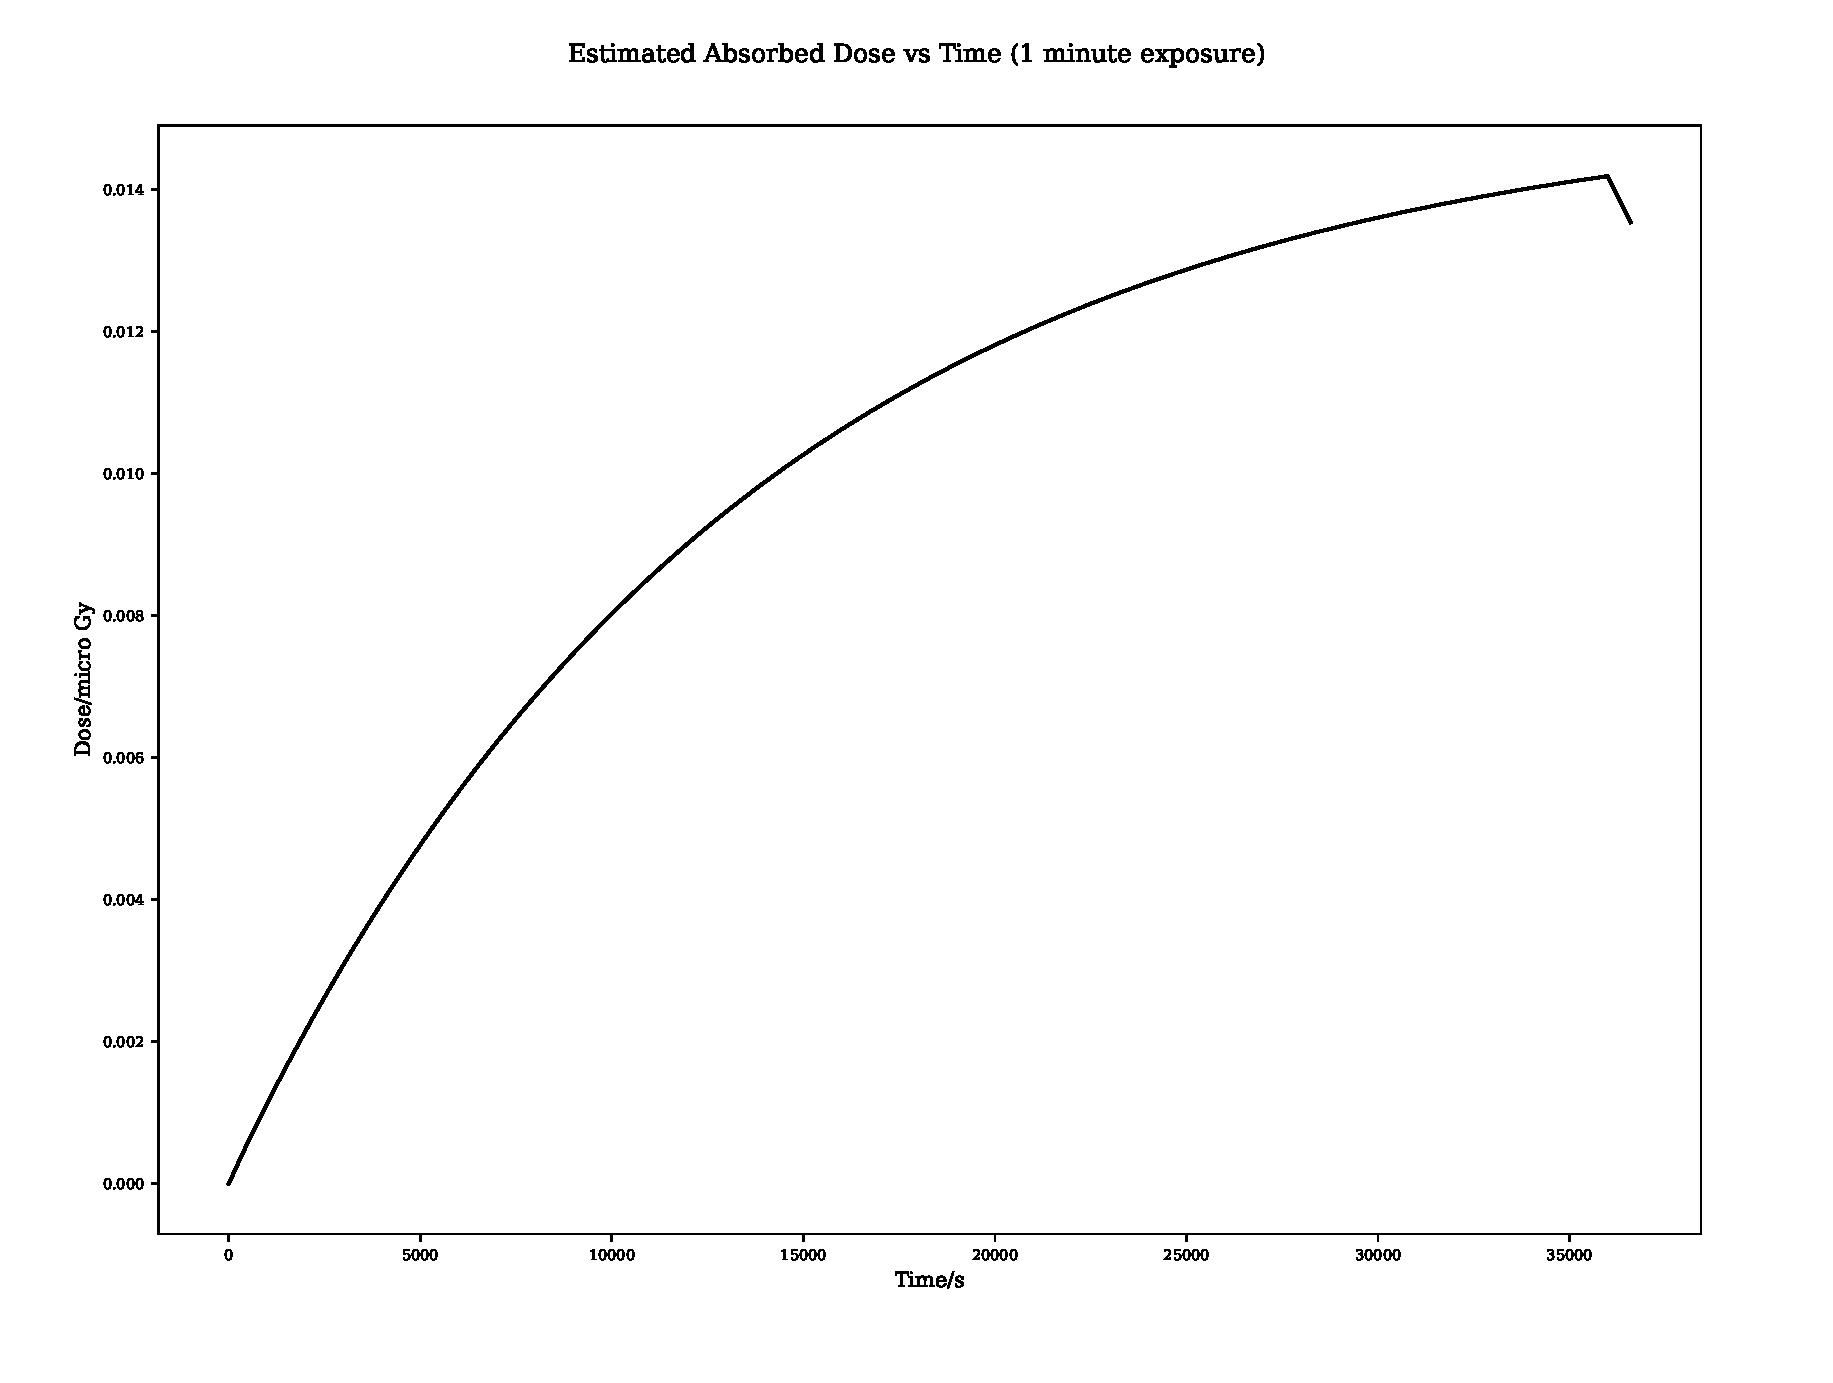
\includegraphics[width=10.0cm]{chapters/background_radiation_effects_and_transport/neutron_plots/1/gamma_dose.eps}
    \captionsetup{font={it}}
    \caption{Steel Irradiation Gamma Dose $2.5 \times 10^7$ neutrons per cm squared per second}
    \label{fig:neutron_irradiated_steel_dose1}
  \end{center}
\end{figure}


\begin{figure}
  \begin{center}
    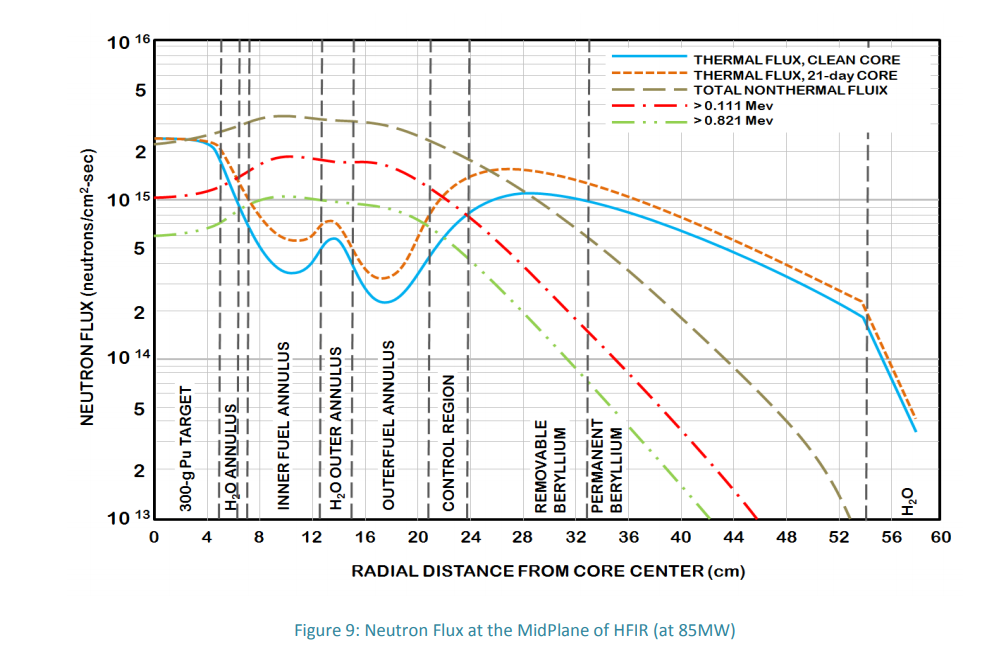
\includegraphics[width=10.0cm]{chapters/background_radiation_effects_and_transport/images/HFIR_neutron_spectra_guide.png}
    \captionsetup{font={it}}
    \caption{High Flux Isotope Reactor Neutron Flux}
    \label{fig:hfir_neutron_flux}
  \end{center}
\end{figure}


\begin{figure}
  \begin{center}
    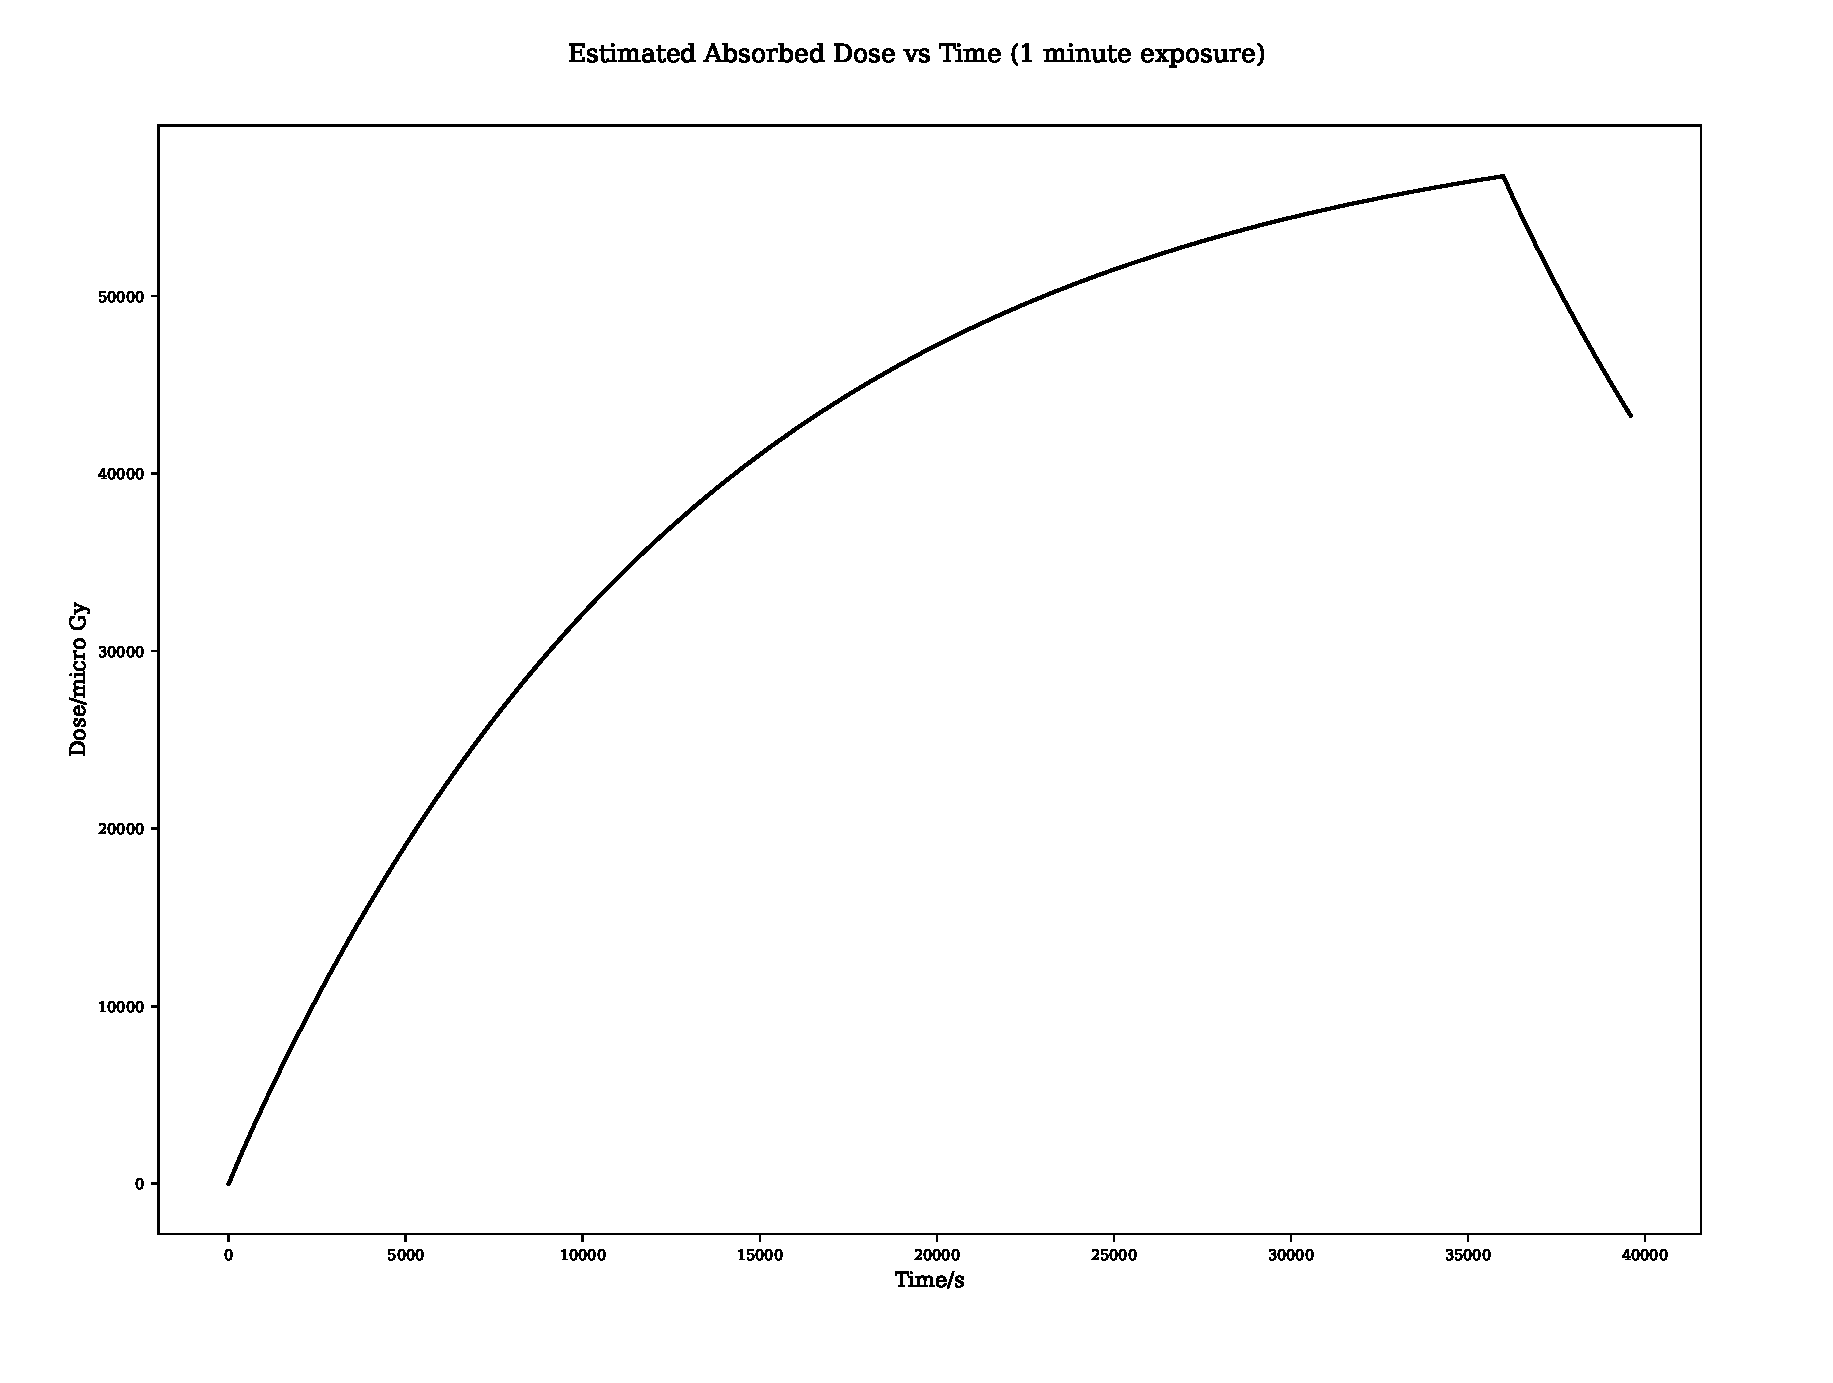
\includegraphics[width=10.0cm]{chapters/background_radiation_effects_and_transport/neutron_plots/2/gamma_dose.eps}
    \captionsetup{font={it}}
    \caption{Steel Irradiation Gamma Dose $1.0 \times 10^{14}$ neutrons per cm squared per second}
    \label{fig:neutron_irradiated_steel_dose2}
  \end{center}
\end{figure}


\FloatBarrier

\subsubsection{Damage to Organics by Radiation}

Life evolved on Earth from single cell to multicelled organisms such as humans.  Prokaryotic cells are single celled organisms that do not have a nucleus, an example being bacteria.  Our cells are eukarytic cells, and these have a nucleus that contains the genetic information.  Millions of cells die in our body every second, and our body replaces these by replicating living cells.  During the replication stage, the DNA within the nucleus is copied.    

DNA is a polymer that is carefully constructed from six components.  Stretched out, it is approximately 2m in length and approximately 25 angstrom wide, and it is neatly contained within the cell nucleus which is on average just 6 microns across.  The structure of DNA is the well known double helix.  The sides of the helix are made from alternating sugars and phosphates, while the \enquote{rungs} of the ladder like structure are pairs of either thymine and adenine or cytosine and guanine.  These pairs are covalently bonded to the sugar-phosphate sides, and by hydrogen bonds to each other.

Mitosis is the part of the cell cycle where the DNA within the nucleus is replicated and the cell splits into two.  There are repair mechanisms, but if the DNA beyond repair, the cell may die through apoptosis, or it may replicate in an uncontrolled way leading to cancer.

Direct damage is caused when ionising radiation alters or destroys sections of DNA through a direct collision, for example a neutron colliding with and knocking out an atom in the DNA strand.

Our cells are predominantly water, so there is a higher probability of the radiation colliding with water molecules than DNA directly.  The chemistry of the contents of the cell is changed, for example by the creation of free radicals, and these lead to damage of DNA as an indirect result of radiation passing through the cell.

\begin{figure}[htb]
\centering
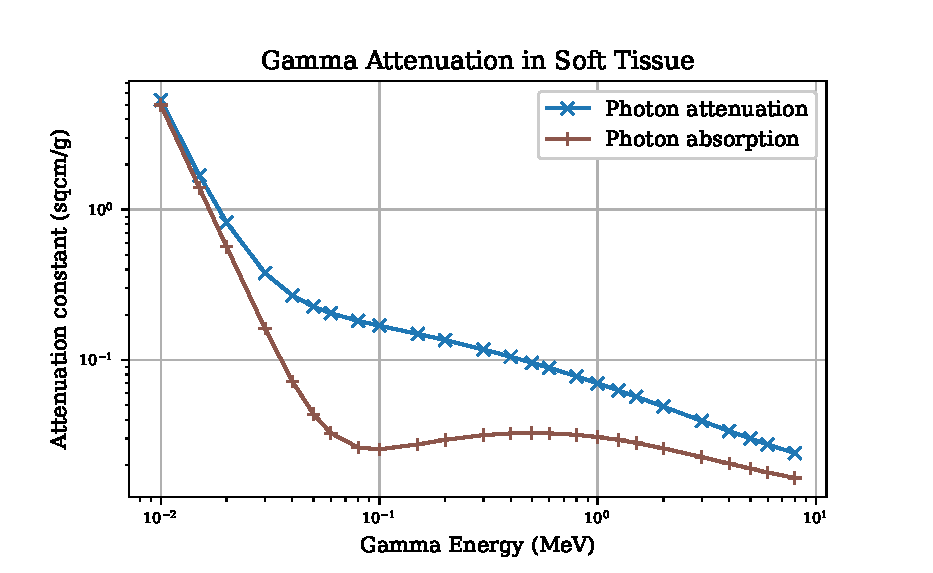
\includegraphics[width=0.5\linewidth]{chapters/background_radiation_effects_and_transport/tissue/soft_tissue_gamma_attenuation.eps}
\caption{.}
\label{fig:softtissueattenuation}
\end{figure}

The damage caused results in either deterministic effects or stochastic effects.  

Where there's a minor exposure to radiation, the damage caused to cells and DNA may lead to cancer later in life, or it may cause issues that are inherited from the irradiated person.  These are stochastic effects as there's a chance they could happen, but it's not certain.

Deterministic effects are due to larger doses where cells are severely damaged.  There's much less chance involved and the effects will be reproduced if multiple people are exposed.  Up to a certain dose, there is still a chance that a person would survive, but the point where the chance of death is 50\% is the \gls{ld50}, and for radiation the dose is 5Sv (table \ref{table:dosecomparison}).

The body relies heavily on three type of blood cell: erythrocytes (red cells), leukocytes (white cells) and thrombocytes (platelets).  These are produced from stem cells within bone marrow and in the course of a day billions are replaced in the body.  Large doses of radiation destroy the cells quicker than they can be produced and this leads to death.  

The lens of the eye is very sensitive to radiation and cataracts can be created by gamma rays.  Radiation can also cause damage to the gut including removal of the lining, bleeding and death.  These are examples of deterministic  effects.

Whilst it is difficult to determine the effects of radiation, particularly for stochastic effects where the effect is heavily dependent on chance, this work on calculating activity of proton irradiated targets aims to give the user a predicted activity and dose value with associated assumptions and caveats.  It is then down to the user to apply the resulting data to the situation and evaluate any health consequences.




%%%%%%%%%%%%%%%%%%%%%%%%%%%%%%%%%%%%%%%%%%%%%%%%%%%%%%%%%%%%%%%%%%%%%%%%%%%%%%%%%%%%%%%%%%%%%%%%%%%%%%%%%%
%%
%%  RADIATION DANGERS
%%
%%%%%%%%%%%%%%%%%%%%%%%%%%%%%%%%%%%%%%%%%%%%%%%%%%%%%%%%%%%%%%%%%%%%%%%%%%%%%%%%%%%%%%%%%%%%%%%%%%%%%%%%%%

\FloatBarrier

\section{Damage Cascades in Metals}

When a metal is damaged by radiation, there are microscopic defects created and removed in a very short space of time.  The result of many months or years of damage is complex and will be discussed in more detail in chapter \ref{chap:backgroundsteels}.

The cohesive energy of atoms are measured in eV (table. \ref{table:cohesiveexamples}), whereas the energy of incoming neutrons or fission fragments are measured in MeV.  Radiation in the form of electrons, protons and heavy ions will lose energy to electrons in the target as they pass through.  They may also lose energy to atoms within the lattice, knocking that atom out of place and creating a \acrshort{pka}.  Due to its neutral charge and magnetic moment, neutrons have a very weak interaction with charged particles.  They primarily lose energy directly with the nucleus of atoms within the target, also creating a \acrshort{pka}.

\begin{table}[h]
\begin{center}
\renewcommand{\arraystretch}{1.2}
\begin{tabular}{c c}
\hline\hline
Element & Cohesive Energy/eV \\
\hline\hline
Aluminium & -3.36 \\
Iron & -4.32 \\
Palladium & -3.91 \\
Platinum & -5.77 \\
Zirconium & -6.32 \\
\hline\hline
\end{tabular}
\end{center}
\caption{Cohesive Energies \cite{shengeamonline}}
\label{table:cohesiveexamples}
\end{table}

The \acrshort{pka}s create a damage cascade, and their mean recoil energy is dependent upon the energy and type of radiation.  After each cascade, there will be a period of time where the material quenches, with a recombination of some interstitials and vacancies.  The \acrshort{pka} creation and cascade thermal spike cover a time range of $10^{-18}$s to $10^{-13}$s, with the quenching phase lasting in the region of $10^{-11}$s.  However, the cumulative effect of radiation damage on a component within a reactor core may only become apparent after months or years.

\begin{table}[h]
\begin{center}
\renewcommand{\arraystretch}{1.2}
\begin{tabular}{c c}
\hline\hline
Projectile & Mean Recoil Energy \\
\hline\hline
1 MeV Electrons & 60eV \\
1 MeV protons & 200eV \\
1 MeV heavy ions & 5keV \\
1 MeV neutrons & 35keV \\
\hline\hline
\end{tabular}
\end{center}
\caption{Average recoil energy of Nickel \acrshort{pka}s\cite{gswas}}
\end{table}

The immediate aftermath of interstitials created three damage cascades is shown in fig. \ref{stollerdamage}.  Damage cascades have been the subject of a number of studies and due to their short time scale and complexity, involving thousands to millions of atoms, are studied with computer simulations.

\begin{figure}
  \begin{center}
    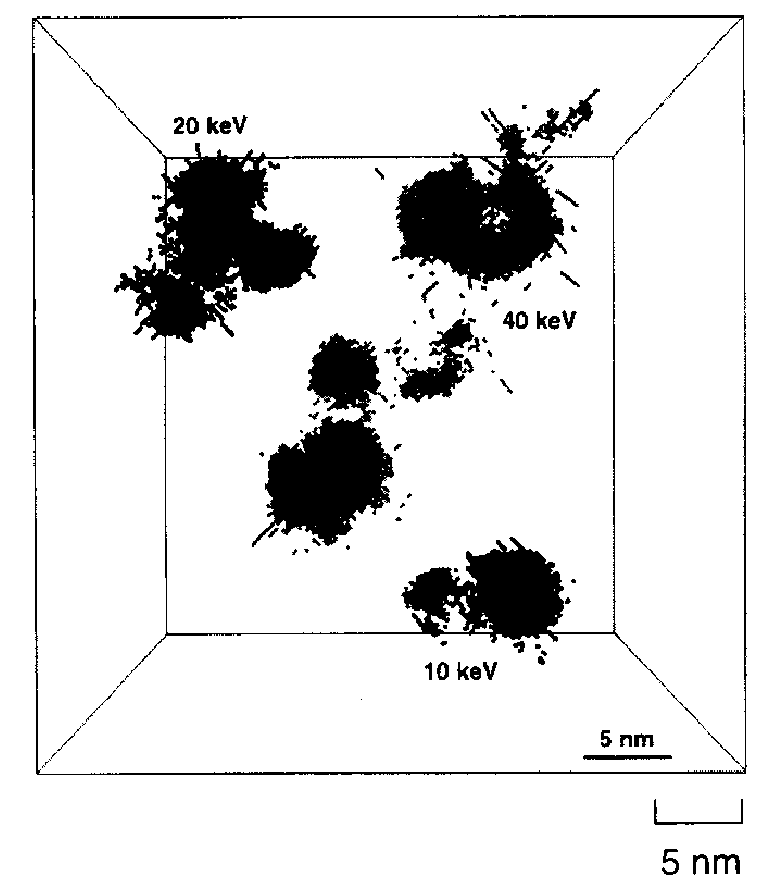
\includegraphics[width=.4\linewidth]{chapters/background_radiation_effects_and_transport/images/stoller1996damage.png}
    \caption{Interstitials in the cascades of 10keV, 20keV and 40keV displacement cascades \cite{stollerdamage1996}}
    \label{fig:stollerdamage}
  \end{center}
\end{figure}


